\documentclass[crop,tikz]{standalone}
\usetikzlibrary{backgrounds}
\colorlet{blue}{cyan}
\tikzset{
  inverted/.style = {
    color=white,
    background rectangle/.style={fill},
    show background rectangle
  }
}

\usepackage{amsmath}
\usepackage{pgfplots}
\usepackage[locale=DE]{siunitx}
\tikzset{>=latex}

\pgfplotsset{
  inverted/.style = {
    every axis legend/.append style={
      draw=white,
      fill=black,
      text=white
    }
  },
  every non boxed x axis/.append style={
    axis line style={-latex}
  },
  every non boxed y axis/.append style={
    axis line style={-latex}
  }
}

\begin{document}
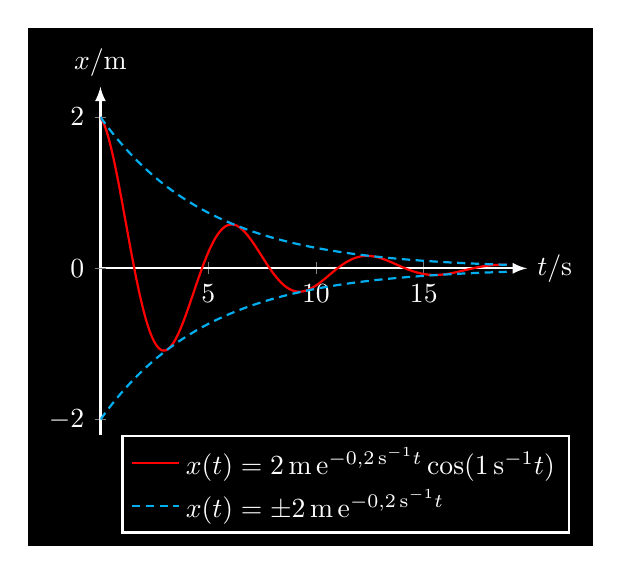
\begin{tikzpicture}[inverted,inverted]
\pgfmathsetmacro{\damp}{0.2}
\begin{axis}[inverted,
  thick,
  width=7cm,
  height=6cm,
  domain={0}:{6*pi},
  samples=100,
  smooth,
  axis y line=middle,
  axis x line=middle,
  xlabel={$t/\si{\s}$},
  ylabel={$x/\si{\m}$},
  xlabel style={right},
  ylabel style={above},
  xmin=0, xmax={6.3*pi},
  ymin=-2.2, ymax=2.4,
  extra y ticks={0},
  legend cell align={left},
  legend style={at={(1.1,0)},anchor=north east}
  ]
  \addplot[red] { 2*exp(-\damp*x)*cos(deg(x)) };
  \addlegendentry{$x(t)=\SI{2}{\m}\operatorname{e}^{-\SI{\damp}{\per\s} t}\cos(\SI{1}{\per\s} t)$};
  \addplot[blue,densely dashed] { 2*exp(-\damp*x) };
  \addlegendentry{$x(t)=\pm\SI{2}{\m}\operatorname{e}^{-\SI{\damp}{\per\s} t}$};
  \addplot[blue,densely dashed] { -2*exp(-\damp*x) };
\end{axis}
\end{tikzpicture}
\end{document}
